\documentclass[../../../main]{subfiles}
\begin{document}

\section{方法}
実験に使用したマイコンユニットは図\ref{fig:micom-unit}で表される。
\begin{figure}
    \begin{small}
        \begin{center}
            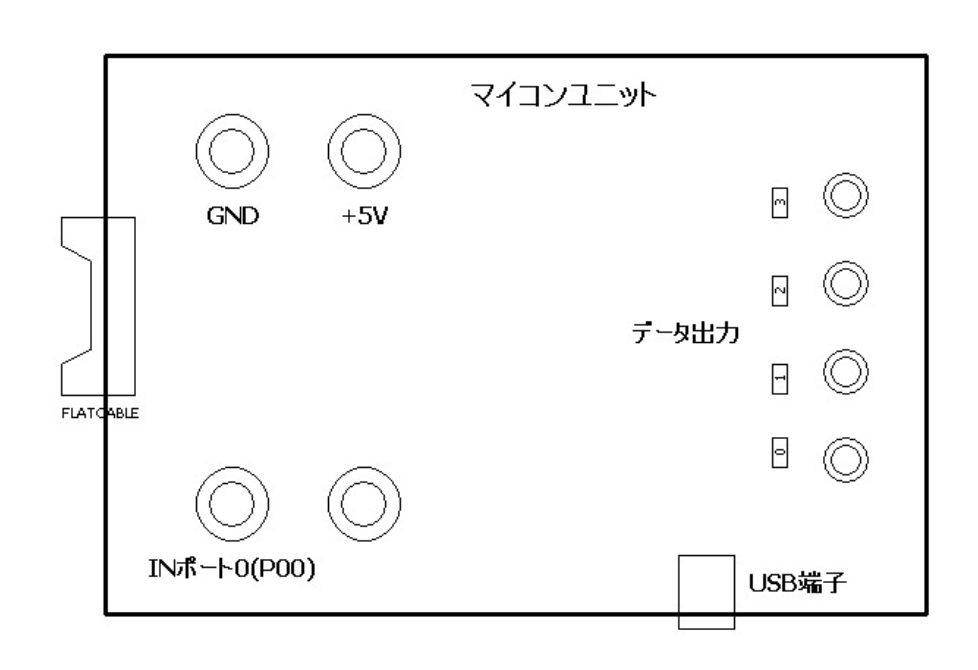
\includegraphics[width=0.95\textwidth]{src/figures/method/micom.png}
        \end{center}
        \caption{マイコンユニット}
        \label{fig:micom-unit}
    \end{small}
\end{figure}


\subsection{実験1}
まず、パソコンのUSB端子とマイコンユニット回路をUSBケーブルで接続した。
次に、マイコンユニット回路の出力信号端子(0~3)とステッピングモータ駆動回路の入力信号端子(0~3)を適当な信号線を用いて接続した。
プログラム(Jikken1.bin)を実行し、キーボードから16進数1桁の数値(0~9およびa~f)を入力すると、その数値がUSBから出力され、マイコンユニット回路を経由し、出力ポートから2進数表現で出力された。
その信号がステッピングモータ駆動回路に送られ、駆動回路の基板上に配置された4つのLEDが入力端子に対応して発光した。
これにより、キーボードからの入力に対応したLEDの点灯状況を確認した。
また、各状態(ON、OFF)の時のマイコンユニット回路の出力電圧を測定した。

\subsection{実験2}
まず、フォトインタラプタ、赤外線距離センサ、超音波距離センサの3種類のセンサを用意した。
最初にフォトインタラプタの特性を計測した。
フォトインタラプタに物を挟んだときと挟まないときのそれぞれの場合の出力電圧を測定した。
測定にはテスターを使用し、電圧が高いときがON、低いときがOFFを表すことを確認した。

次に、赤外線距離センサの特性を計測した。
赤外線センサからの発光(赤外線)を障害物に当てて反射させ、その反射信号の強度によってセンサと障害物の距離を計測した。
赤外線センサの出力は電圧であり、受光強度によって変化するため、障害物までの距離を物差しで測定し、センサ信号電圧をテスターで測定した。
その結果を用いて横軸を距離、縦軸をセンサ出力(電圧)とするグラフを作成した。

最後に、超音波距離センサの特性を計測した。
超音波センサから出される超音波を障害物に当てて反射させ、その反射波の状態によってセンサと障害物の距離を計測した。
超音波センサでは12Vの電圧が必要であるため、配線に注意した。
超音波センサの出力信号はパルス波となっており、センサと障害物の距離によってパルス幅が変化するため、オシロスコープで出力を表示し、パルス一つあたりの幅を読み取った。
その結果を用いて横軸を距離、縦軸をパルス幅とするグラフを作成した。

\subsection{実験3}
まず、フォトインタラプタの出力端子とマイコンユニット回路のP00ポートの端子を接続した。
フォトインタラプタの実験では、センサに物を挟んだときと挟まないときそれぞれでON-OFFの出力が得られた。
プログラム(Jikken31.bin)を実行し、ONのときに「input data exists」、OFFのときに「no input data」という表示がパソコンの画面に現れることを確認した。
表示された結果が実験2(1)のセンサ出力の対応関係と一致していることも調べた。

次に、赤外線センサの出力端子とマイコン回路のP00ポートの端子を接続した。
赤外線距離センサについては、センサと障害物の距離を少しずつ変えていったときに、画面上の表示がどうなるかについて調べた。
フォトインタラプタと同様に、パソコン画面の表示は「input data exists」「no input data」であり、センサ-障害物間の距離と表示がどう対応するかをまとめた。
実験2(2)の結果とこの実験結果から、マイコンユニット回路内のON-OFFの閾値が何Vくらいに設定されているかを考えた。

最後に、超音波センサの出力端子とマイコンユニット回路のP00ポートの端子を接続した。
プログラム(Jikken33.bin)を実行し、マイコンに入力された超音波センサの出力パルス信号のパルス幅をある時間間隔でカウントするようにした。
センサと障害物の距離を少しずつ変えていったときに画面に表示されるカウント数を調べ、その結果を用いて横軸を距離、縦軸をパルス幅カウント数とするグラフを作成した。
このグラフが実験2(3)のグラフと同形になることを確認した。

\subsection{実験4}
まず、マイコンユニット回路、ステッピングモータ駆動回路、ステッピングモータをそれぞれ正しく接続した。
次に、プログラム(Jikken4.bin)を実行し、適当なステップ数、回転速度、回転方向を入力した。
モータが回転している時間をストップウォッチで測定し、1ステップあたり7.5度回転することを利用して回転速度を計算した。

次に、モータが回転しているときの各端子の信号をオシロスコープで観察し、スケッチした。
モータ駆動回路からモータに送られている4つの信号をオシロスコープに表示し、各波形の位相の状態までわかるようにした。
波形のパルス幅や電圧レベルも含めて詳細にスケッチした。

さらに、オシロスコープで観察されたステッピングモータ駆動パルスから、1ステップあたりの時間を求めた。
1ステップの時間と1ステップあたりの回転角(7.5度)を用いて回転速度を計算した。

最後に、ストップウォッチで測定した回転速度とオシロスコープで観察した回転速度を比較した。
これにより、2種類の方法で求めた計算速度の整合性を確認した。


\subsection{実験5}

まず、実験4の配線を保ったままで、それぞれのセンサ出力端子とマイコンユニット回路のP00ポートの端子を接続した。
各センサを配線したときの制御の様子を観察した。

最初にフォトインタラプタを用いた総合実験を行った。
ステッピングモータに取り付けた円盤がフォトインタラプタのセンサ部分に挟まるように設置した。
プログラム(Jikken51.bin)を実行し、穴の数と回転方向を入力した。
円盤上の穴の数が4つであるため、4の倍数を入力すると分かりやすかった。
回転速度を遅くすることで読み飛ばしなどの誤動作を防ぎ、観察した結果をまとめた。

次に、赤外線センサを用いた総合実験を行った。
フォトインタラプタと赤外線センサを置き換えて配線し、プログラム(Jikken52.bin)を実行した。
回転方向を入力し、センサと障害物の距離を少しずつ変えていったときに、回転が止まったときのセンサと障害物の距離を測定した。
この結果を実験3(2)で求めたマイコンユニット回路における信号のON-OFF基準と比較して確認した。

最後に、超音波センサを用いた総合実験を行った。
赤外線センサと超音波センサを置き換えて配線し、超音波センサには12Vの電圧が必要であるため配線に注意した。
プログラム(Jikken53.bin)を実行し、パルスカウント数と回転方向を入力した。
センサパルスの幅をカウントし、そのカウント数が指定したパルスカウント数よりも小さくなったときにモータが停止するように設定した。
センサと障害物の距離を少しずつ変えていき、モータが止まったときの距離を測定した。
この結果を実験3(3)の結果と比較してモータの制御が適切に行われているかを確認した。


\end{document}
